\documentclass[class=report, crop=false, 12pt,a4paper]{standalone}
\usepackage{enumitem}
\usepackage{multicol}
\usepackage{etoolbox}
\AtBeginEnvironment{quote}{\singlespacing\small}
\usepackage{setspace}
\onehalfspacing
\usepackage{graphicx}
\usepackage{siunitx}
\sisetup{detect-all}
\begin{document}
\section{Fluid Properties}
Fluids have many properties including:

\begin{multicols}{2}
  \begin{itemize}[noitemsep]
    \item Surface Tension - \( \sigma \).
    \item Viscosity - \( \mu \).
    \item Compressibility.
    \item Density \( \rho \).
    \item Temperature.
    \item Pressure - P.
  \end{itemize}
\end{multicols}

What is a fluid?
\begin{quote}
  \begin{center}
    A fluid is a substance that deforms continuously when acted on by a shearing stress of any magnitude. 
  \end{center}
\end{quote}
This includes gases and liquids but not silly putty, gels or glass. Some soft materials such as toothpaste will only start to flow once a critical shear stress has been reached. This is the study of rheology and not studied in this module.

In classical fluid mechanics, we treat fluids as a continuum because there is an extremely large number of particles. Thus, we can conclude that fluid parameter such as pressure and density vary continuously throughout the fluid.

\subsection{Shear strain for solid bodies}
What is shear strain?
\begin{quote}
  \begin{center}
    Shear strain is the change in angle as an element experience a force tangential to its surface.
  \end{center}
\end{quote}
\begin{center}
  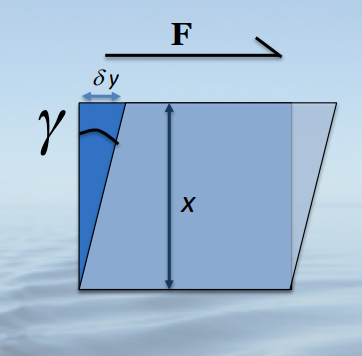
\includegraphics[width = 0.4 \textwidth]{../img/ShearStrainDiagram}
\end{center}
For a fluid, we are interested in the rate of shear. A specific tangential force will cause a fixed amount of shear strain per unit time. If the speed of the top layer is \( u_y\), the shear rate is \(\delta u_y / \delta x\).
\begin{equation}
  tan(\gamma) = \frac{\delta y}{x} \approx \gamma
\end{equation}

\subsection{Shear stress on a solid body}
For a solid, the shear force is the force applied tangentially to a surface.

\emph{Shear stress} is the tangential force per unit area \( \tau\).

\emph{Normal stress} is the perpendicular force per unit area \( \sigma \).

\begin{center}
  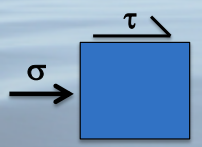
\includegraphics[width = 0.4 \textwidth]{../img/ShearForceDiagram}
\end{center}

\subsection{Simple laminar flow case}
Consider flat layers of fluid sliding over each other. The sideways velocity of the fluid changes as you move away from the stationary boundary. The velocity of the y direction, \( u_y \) is changing with position, \( x\). 

\begin{center}
  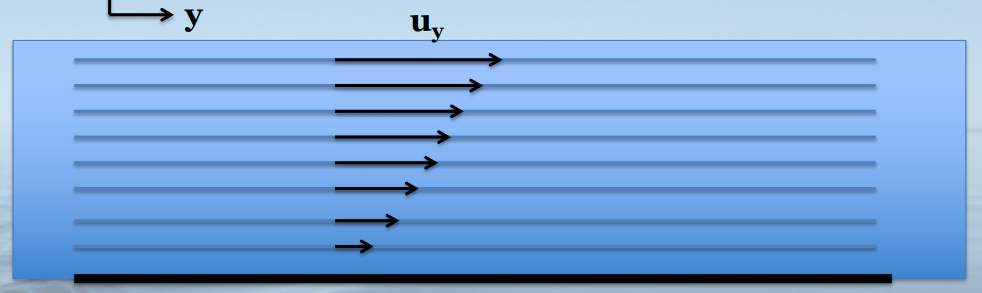
\includegraphics[width = 1 \textwidth]{../img/LaminarFlowSimple}
\end{center}

\subsection{Viscosity}
\begin{equation}
  \tau = \mu \frac{du_y}{dx}
\end{equation}
Where:
\begin{multicols}{2}
  \begin{itemize}[noitemsep]
    \item \(\tau \) = Shear stress = force/area.
    \item \(\mu \) = Dynamic viscosity.
    \item \( du_y / dx \) = Shear rate.
    \item Units: Velocity change per unit perpendicular distance.
  \end{itemize}
\end{multicols}
Viscosity is the constant of proportionality, telling us how much shear stress is required to produce a given shear rate. Shear stress can be different at different places in the same fluid. Equation (2) is Newton's equation for viscosity and he assumed that the viscosity was a constant. However, this is not always true and the fluids for which that does not apply are called \emph{non-Newtonian fluids.} An example of a shear \emph{thickening} fluid is corn-starch, i.e. viscosity increases with shear rate. An example of shear \emph{thinning} fluid is blood or ketchup, i.e. viscosity decreases with shear rate. We cannot use laminar flow analysis to study blood vessels because they constrict and dilate as fluids pass through - the rigid boundary condition does not apply (or you would not be able to feel your pulse.) We will only be studying Newtonian fluids and rigid boundaries.

Viscosity changes as a function of temperature and pressure. In liquids, when the temperature increases, the viscosity decreases. In gases, the reverse occurs, with viscosity increasing with temperature. Relatively, pressure has a weak effect on the viscosity of a fluid.

The standard symbol for the viscosity as defined above is \( \mu \) and this is known as the \emph{dynamic viscosity} (ratio of shear stress to the the shear rate) with units \si{\kg\per\meter\per\second} or \si{\pascal \second}. This will be our definition of viscosity. For some applications it is easier to do calculations in terms of the viscosity per unit density:
\begin{equation}
  v = \frac{\mu}{\rho}
\end{equation}

\subsection{Surface tension}
What is surface tension?
\begin{quote}
  \begin{center}
    Surface tension is the effective tangential force per unit length (\si{\newton\per\meter}) exerted on an imaginary line through a surface, due to intermolecular interaction.
  \end{center}
\end{quote}

Surface tension is always considered perpendicular to the line it's pulling on. In this case, we want the force exerted on the thread. If the thread has length L, the total force on one side of the soap film is \(\sigma L\), so the total force from both sides is \(2\sigma L\).
\begin{center}
  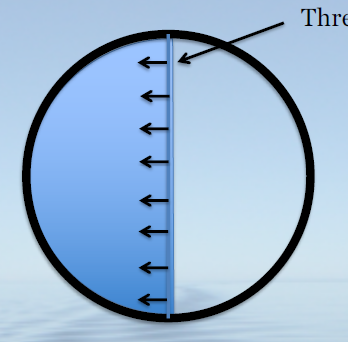
\includegraphics[width = 0.4 \textwidth]{../img/SoapFilm}
\end{center}
Surface tension is what allows a drop of liquid to take its unique shape, when there are no external forces present.

\subsection{Capillary action}
This is caused by two processes:
\begin{itemize}[noitemsep]
  \item \emph{Adhesion} between the water molecules and the tube wall.
  \item \emph{Cohesion} between water molecules.
\end{itemize}
However, the surface tension (cohesion) must still be strong enough to drag the fluid up the pipe. When the angle of contact between a solid and a liquid is 90 degrees, then the cohesive force = the adhesive force.
\begin{center}
  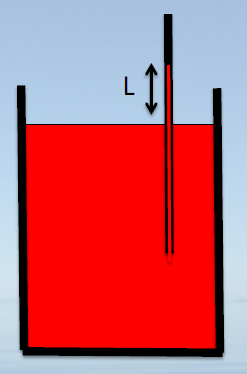
\includegraphics[width = 0.4 \textwidth]{../img/CapillaryAction}
\end{center}
The liquid will rise by itself up the tube and this gives us a crude method for calculating surface tension. The weight of the water must be balanced by the surface tension forces at the water surface.
\begin{equation}
  F = 2\pi \sigma = L\pi r^2 \rho g
\end{equation}
\begin{equation}
  \sigma = \frac{1}{2}\rho r g L
\end{equation}

\subsection{Pressure}
What is Pascal's Law?
\begin{quote}
  \begin{center}
    The pressure at a point in a fluid at rest or in motion is independent of direction as long as there are no shearing forces present.
  \end{center}
\end{quote}
The volume of a fluid under pressure will depend on the magnitude of the pressure. However, for many liquids (e.g. water), the change in volume is so small that it can be considered \emph{negligible.} Even in everyday situations, water obviously is not really incompressible because sound waves can travel through it. For a truly incompressible fluid, the speed of sound would be infinite. Seawater density varies with temperature, pressure and salinity but below the top one kilometre, where salinity and temperature are nearly uniform, there is almost no variation in density with depth. The relationship between the pressure, volume and temperature of a fluid is described by an \emph{equation of state}. Any equation that relates pressure and volume tells us something about the compressibility of a fluid. Pressure is also the same in all directions from our continuum assumption.
\begin{center}
  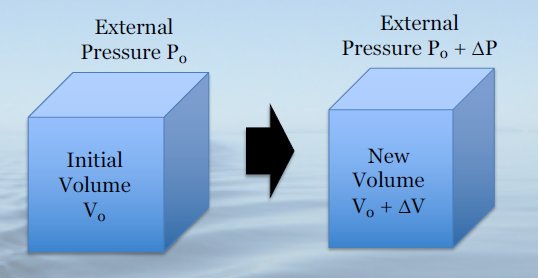
\includegraphics[width = 0.8 \textwidth]{../img/CompressibilityOfFluid}
\end{center}
We are interested in finding \( dV/dP\) which is (almost) always negative. A fluid is considered \emph{compressible} when its volume varies significantly with temperature and pressure in the parameter space of interest. If there is no significant variation, the fluid can be considered \emph{incompressible}. We will only be covering compressible fluids.

\subsection{Example Question: Cartesian diver}
Consider a closed vessel that is completely full of water but with flexible sides (plastic bottle). Inside is a cylinder that is closed at the top but open at the bottom. It is partly full of air and has some extra mass added at the base. The plastic parts of the diver have a volume of \(1.067\times 10^{-6} \) \si{\meter\cubed} and a density of \(2400\) \si{\kg\per\meter\cubed}. At atmospheric pressure, the length of the air column is 1.5 \si{\cm} and the cross-sectional area is \(1\times 10^{-4}\) \si{\meter\squared}. The temperature in the room is \(20^{\circ}\)C. 

Question: How much pressure must be applied to the bottle to make the diver sink?

We must ask an important question: is the total density of the diver and the air and the water greater than or less than the density of the water around it? We know that \( \rho_w = 1000\) \si{kg\per\meter\cubed} and if the water is compressible, the total density of the whole diver is given by:
\[ \rho_D = \frac{\rho_A l_1 A + \rho_w l_2 A + M_D}{(l_1 + l_2)A} \]
Where \(M_D\) is the mass of the plastic parts of the diver. 
\begin{center}
  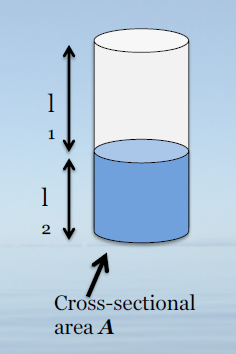
\includegraphics[width = 0.4 \textwidth]{../img/CartesianDiver}
\end{center}
We can see that the diver will sink if \(\rho_D > \rho_w\) and it rises if \(\rho_D < \rho_w\).

Method: set the densities to be equal and deduce an expression for the pressure in this situation. 
\[ \rho_w = \rho_D = \frac{\rho_A l_1 A + \rho_w l_2 A + \rho_P V_P}{(l_1 + l_2)A + V_P} \]
To calculate the density of air, we need the equation of state. Assume that \( R_g = 287\) \si{\joule\per\kg\per\kelvin}
\[ P = \rho_A R_g T\]
The necessary pressure is determined by the necessary density of air. So, we start by rearranging the equation to specify the density of air. 
\[ \rho_A = \frac{1}{l_1 A} \left( \rho_w \left( (l_1 + l_2)A + V_P \right) - \rho_w l_2 A - \rho_P V_P \right)\]
\[ \rho_A = \frac{1}{l_1 A} \left( \rho_w \left( (l_1A + V_P) \right) -\rho_P V_P \right) \]
We can now use the equation of state to find an expression for the pressure. 
\[ P = \frac{R_g T}{l_1 A} \left( \rho_w \left( (l_1A + V_P) \right) -\rho_P V_P \right) \]
From here we can substitute our values to arrive at an answer of \( P = 3.48 \times 10^5\) \si{\newton\per\meter\squared} or approximately 3.5 atmospheres. 

In many situations, we assume  that liquids are incompressible. However, this is an \emph{assumption} that must be justified. 

\section{Buoyancy and stability}
The resultant force acts at the centre of gravity of the fluid, the centroid of the volume. This is called the centre of buoyancy. Whatever is filling the space also has a force acting on it: it's weight. This acts at its centre of mass. The resultant force is given by: 
\begin{equation}
  F_\uparrow - F_\downarrow = (\rho_w - \rho_0) give
\end{equation}
\begin{center}
  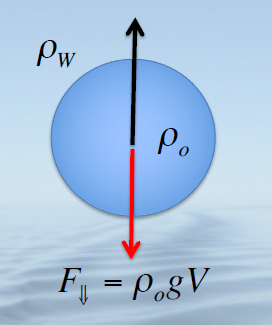
\includegraphics[width = 0.4 \textwidth]{../img/BuoyancyForces}
\end{center}
An object is neutrally buoyant if the weight and the buoyant forces are equal, so the system is in equilibrium. INSERT EXAMPLE MERT

\subsection{Instability}
Consider a submerged ping pong ball which is half filled with plasticine and the other half just filled with air.
\begin{center}
  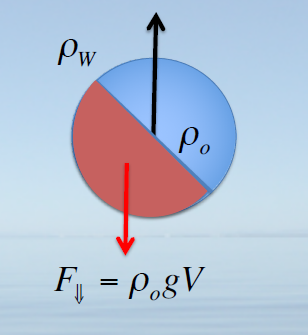
\includegraphics[width = 0.4 \textwidth]{../img/InstabilityPingPong}
\end{center}
Assume that the ball overall is neutrally buoyant. The forces are equal and opposite but there is a \emph{couple}. The ball will rotate in response to the couple until the forces are aligned. At this point, the object is stable. The buoyancy and the weight do not necessarily have the same line of action. We must also consider whether the object will maintain its orientation. 
\begin{itemize}
  \item \emph{Stable} equilibrium: when displaced slightly, there is a net force acting to push the object back to its initial orientation.
  \item \emph{Unstable} equilibrium: when displaced slightly, there is a net force acting to push the object further from its initial orientation.
  \item \emph{Neutral} equilibrium: when displaced slightly, there is no net force. 
\end{itemize}
If the centre of buoyancy is above the centre of gravity, the object is in a stable equilibrium. 
\subsection{Centre of mass}
The centre of mass is calculated in an analogous way to the centroid of the volume. If we split any object in half with a flat plane that passes through its centre of mass, there will be equal mass in both halves.
\[ x_{CoM} = \frac{1}{m}\int_m x dm \]
\[ y_{CoM} = \frac{1}{m}\int_m y dm \]
\[ z_{CoM} = \frac{1}{m}\int_m z dm \]
Where m is the total mass of the object. 

In a semi-submerged body, the upward thrust is equal to the weight of the \emph{displaced} fluid. For a body to be in vertical equilibrium, the immersed body must generate a buoyancy force equal and opposite to the weight of the object.
\end{document}